\documentclass{beamer}
%\title{text}
%\author{text}
%\date{date}
\usetheme{Boadilla}
\definecolor{blue(munsell)}{rgb}{0.0, 0.5, 0.69}
\definecolor{blue(ryb)}{rgb}{0.01, 0.28, 1.0}
\definecolor{blizzardblue}{rgb}{0.67, 0.9, 0.93}
\definecolor{green(pigment)}{rgb}{0.0, 0.65, 0.31}
\definecolor{green(html/cssgreen)}{rgb}{0.0, 0.5, 0.0}
\usepackage{tikz}
\usetikzlibrary{mindmap,trees}
\usepackage{verbatim}
\usepackage{adjustbox}
\usepackage[utf8]{inputenc} % diacritice

\begin{document}

\begin{frame}{MINDMAP}
\resizebox{\textwidth}{!}{
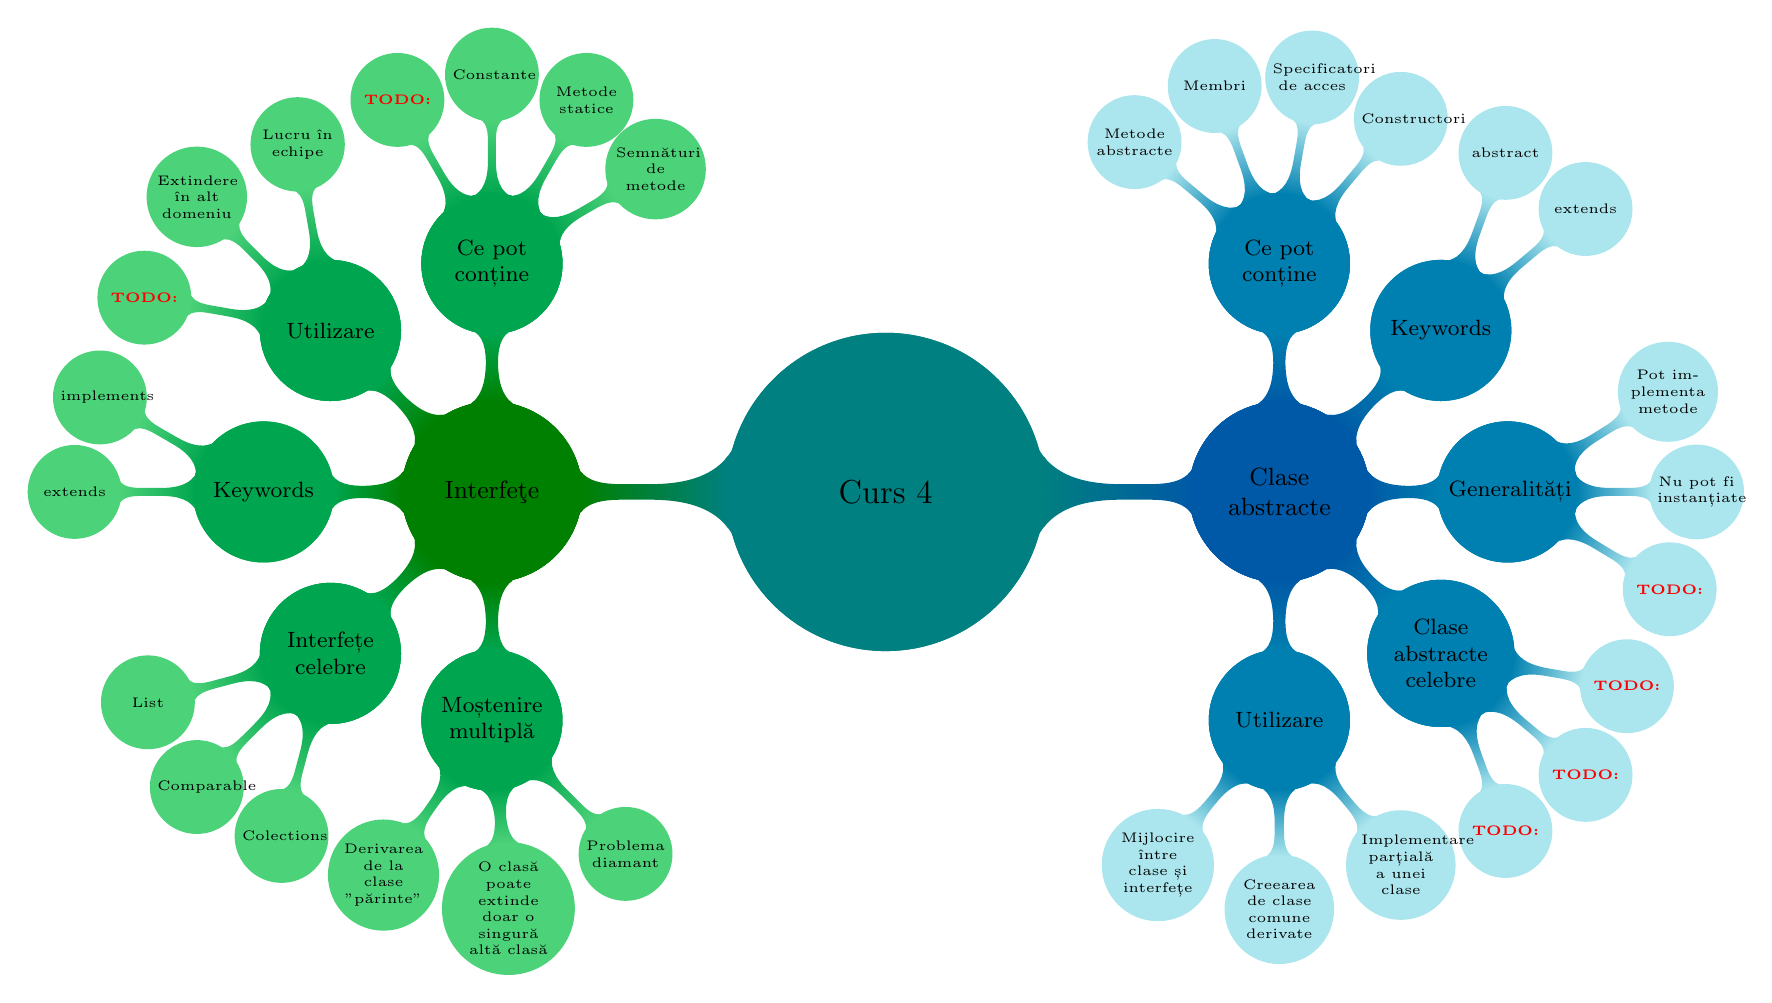
\begin{tikzpicture}
 	\path[mindmap, concept color=teal,text=black]
	node[concept] {Curs 4} [clockwise from=0]
	child[concept color = blue!30!teal] {
		node[concept] {Clase abstracte}[clockwise from=45]
		child[concept color = blue(munsell)] {
			node[concept] {Keywords}[clockwise from=70] {
				child[concept color = blizzardblue]{
					node[concept]{abstract}
				}
			}
			node[concept] {Keywords}[clockwise from=40] {
				child[concept color = blizzardblue]{
					node[concept]{extends}
				}
			}
		}		
		node[concept] {Clase abstracte}[clockwise from=90]
		child[concept color = blue(munsell)] {
			node[concept] {Ce pot conține}[clockwise from=140] {
				child[concept color = blizzardblue]{
					node[concept]{Metode abstracte}
				}
			}
			node[concept] {Ce pot conține}[clockwise from=110] {
				child[concept color = blizzardblue]{
					node[concept]{Membri}
				}
			}
			node[concept] {Ce pot conține}[clockwise from=80] {
				child[concept color = blizzardblue]{
					node[concept]{Specificatori de acces}
				}
			}
			node[concept] {Ce pot conține}[clockwise from=50] {
				child[concept color = blizzardblue]{
					node[concept]{Constructori}
				}
			}
		}	
		node[concept] {Clase abstracte}[clockwise from=0]
		child[concept color = blue(munsell)]{
			node[concept] {Generalități}[clockwise from = 32] {
				child[concept color = blizzardblue]{
					node[concept]{Pot implementa metode}
				}
			}
			node[concept] {Generalități}[clockwise from = 0] {
				child[concept color = blizzardblue]{
					node[concept]{Nu pot fi instanțiate}
				}
			}
			node[concept] {Generalități}[clockwise from = -31] {
				child[concept color = blizzardblue]{
					node[concept, text = red]{\textbf{TODO:}}	
				}
			}
		}
		node[concept] {Clase abstracte}[clockwise from=-45]
		child[concept color = blue(munsell)] {
			node[concept]{Clase abstracte celebre}[clockwise from = -10] {	
				child[concept color = blizzardblue]{
					node[concept, text = red]{\textbf{TODO:}}	
				}
			}
			node[concept]{Clase abstracte celebre}[clockwise from = -40] {
				child[concept color = blizzardblue]{
					node[concept, text = red]{\textbf{TODO:}}
				}
			}
			node[concept]{Clase abstracte celebre}[clockwise from = -70] {
				child[concept color = blizzardblue]{
					node[concept, text = red]{\textbf{TODO:}}
				}
			}
		}
		node[concept] {Clase abstracte} [clockwise from=-90]
		child[concept color = blue(munsell)]{
			node[concept]{Utilizare}[clockwise from = -50] {
				child[concept color = blizzardblue]{
					node[concept]{Implementare parțială a unei clase}
				}
			}
			node[concept]{Utilizare}[clockwise from = -90] {
				child[concept color = blizzardblue]{
					node[concept]{Creearea de clase comune derivate}
				}
			}		
			node[concept]{Utilizare}[clockwise from = -130] {
				child[concept color = blizzardblue]{
					node[concept]{Mijlocire între clase și interfețe}	
				}
			}
		}
	}
	node[concept] {Curs 4} [clockwise from=180]
	child[concept color = green(html/cssgreen)] {
		node[concept] {Interfețe} [clockwise from=90]
		child[concept color = green(pigment)]{
			node[concept]{Ce pot conține}[clockwise from = 30] {
				child[concept color = green!50!teal!70!white] {
					node[concept]{Semnături de metode}
				}
			}
			node[concept]{Ce pot conține}[clockwise from = 60]{
				child[concept color = green!50!teal!70!white]{
					node[concept]{Metode statice}
				}
			}
			node[concept]{Ce pot conține}[clockwise from = 90]{
				child[concept color = green!50!teal!70!white]{
					node[concept]{Constante}
				}
			}
			node[concept]{Ce pot conține}[clockwise from = 120]{
				child[concept color = green!50!teal!70!white]{
					node[concept, text = red]{\textbf{TODO:}}
				}
			}
		}
		node[concept] {Interfețe} [clockwise from=135]
		child[concept color = green(pigment)]{
			node[concept] {Utilizare} [clockwise from = 100] {
				child[concept color = green!50!teal!70!white]{
					node[concept]{Lucru în echipe}
				}
			}
			node[concept] {Utilizare} [clockwise from = 135] {
				child[concept color = green!50!teal!70!white]{
					node[concept]{Extindere în alt domeniu}
				}
			}
			node[concept] {Utilizare} [clockwise from = 170] {
				child[concept color = green!50!teal!70!white]{
					node[concept, text = red]{\textbf{TODO:}}
				}
			}
		}	
		node[concept] {Interfețe} [clockwise from=180] 
		child[concept color = green(pigment)]{
			node[concept] {Keywords} [clockwise from = 150] {
				child[concept color = green!50!teal!70!white]{
					node[concept]{implements}
				}
			}
			node[concept] {Keywords} [clockwise from = 180] {
				child[concept color = green!50!teal!70!white]{
					node[concept]{extends}
				}
			}				
		}
		node[concept] {Interfețe} [clockwise from=225]
			child[concept color = green(pigment)]{
				node[concept] {Interfețe celebre} [clockwise from = 195] {
					child[concept color = green!50!teal!70!white]{
						node[concept]{List}
					}
				}
				node[concept] {Interfețe celebre} [clockwise from = 225] {
					child[concept color = green!50!teal!70!white]{
						node[concept]{Comparable}	
					}
				}
				node[concept] {Interfețe celebre} [clockwise from = 255] {
					child[concept color = green!50!teal!70!white]{
						node[concept]{Colections}
					}
				}
		}
		node[concept] {Interfe\c te} [clockwise from=270]
		child[concept color = green(pigment)]{
			node[concept] {Moștenire multiplă} [clockwise from=235] {
				child[concept color = green!50!teal!70!white]{
					node[concept]{Derivarea de la clase "părinte"}
				}
			}
			node[concept] {Moștenire multiplă} [clockwise from=275] {
				child[concept color = green!50!teal!70!white]{
					node[concept]{O clasă poate extinde doar o singură altă clasă}
				}
			}
			node[concept] {Moștenire multiplă} [clockwise from=315] {
				child[concept color = green!50!teal!70!white]{
					node[concept]{Problema diamant}
				}
			}
		}
	};
\end{tikzpicture}
}
\end{frame}
\end{document}
